\documentclass[11pt]{article}
\usepackage[utf8]{inputenc}
\usepackage[T1]{fontenc}
\usepackage{amsmath}
\usepackage{amssymb}
\usepackage{multicol}
\usepackage{geometry}
\usepackage{tikz}
\usepackage{enumitem}
\usepackage{xcolor}
\usepackage{titlesec}

% Configurações de layout
\geometry{a4paper, left=1cm, right=1cm, top=0.5cm, bottom=1.2cm}
\setlength{\columnseprule}{0.4pt}

% Cores para títulos
\titleformat{\section}{\normalfont\Large\bfseries\color{blue}}{\thesection}{1em}{}
\titleformat{\subsection}{\normalfont\large\bfseries\color{red}}{\thesubsection}{1em}{}

\title{\textcolor{blue}{Tecnologia e Cidadania Digital
    \\Cibersegurança e Ética Digital}}
\author{Professor: Jefferson}
\date{}

\begin{document}

\maketitle
\vspace{-1cm}

\begin{center}
\large{Nome: \underline{\hspace{8cm}} \quad Turma: \underline{\hspace{3cm}}}
\end{center}

\begin{multicols}{2}

\section*{Conceitos Fundamentais}

\subsection*{Cibersegurança}

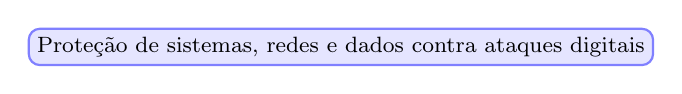
\begin{tikzpicture}
\node[rectangle, fill=blue!10, rounded corners, inner sep=3pt, draw=blue!50, thick] (box) {
\footnotesize Proteção de sistemas, redes e dados contra ataques digitais
};
\end{tikzpicture}

\textbf{Pilares:}
\begin{itemize}
\item Confidencialidade
\item Integridade
\item Disponibilidade
\item Autenticidade
\end{itemize}

\subsection*{Ética Digital}

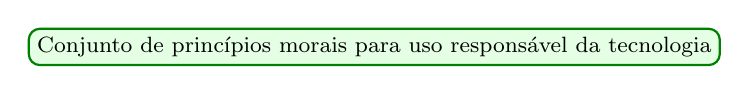
\begin{tikzpicture}
\node[rectangle, fill=green!10, rounded corners, inner sep=3pt, draw=green!50!black, thick] (box) {
    \footnotesize
Conjunto de princípios morais para uso responsável da tecnologia
};
\end{tikzpicture}

\textbf{Princípios:}
\begin{itemize}
\item Respeito à privacidade
\item Honestidade online
\item Responsabilidade pelas ações
\item Respeito aos direitos autorais
\end{itemize}


\section*{Exercícios}

\begin{enumerate}[leftmargin=*]

\item \textbf{Senhas Seguras:}
\begin{enumerate}[label=\alph*)]
\item Quais características tornam uma senha forte?
\item Por que não devemos usar a mesma senha em vários serviços?
\item Crie uma senha forte seguindo as boas práticas
\end{enumerate}


\item \textbf{Redes Sociais - Analise situações:}
\begin{enumerate}[label=\alph*)]
\item Um amigo posta foto sua sem sua permissão. O que fazer?
\item Você encontra informações falsas sobre um colega. Qual sua atitude?
\item É ético criar perfil falso para "investigar" alguém?
\end{enumerate}

\item \textbf{Direitos Autorais:}
\begin{enumerate}[label=\alph*)]
\item Você pode usar qualquer imagem da internet em seu trabalho escolar?
\item Como identificar conteúdo com licença livre?
\item O que é plágio e como evitá-lo?
\end{enumerate}

\item \textbf{Privacidade vs. Compartilhamento:}
\begin{enumerate}[label=\alph*)]
\item Quais informações pessoais nunca devem ser compartilhadas online?
\item Como configurar a privacidade nas redes sociais?
\item Quais os riscos de compartilhar localização em tempo real?
\end{enumerate}

\item \textbf{Cyberbullying:}
\begin{enumerate}[label=\alph*)]
\item Defina cyberbullying e dê exemplos
\item Qual deve ser a atitude de uma vítima?
\item Como ser um espectador proativo?
\end{enumerate}

\item \textbf{Backup e Proteção:}
\begin{enumerate}[label=\alph*)]
\item Por que fazer backup regular dos dados?
\item Quais dispositivos precisam de antivírus?
\item O que é autenticação em dois fatores e por que usar?
\end{enumerate}

\item \textbf{Compras Online Seguras:}
\begin{enumerate}[label=\alph*)]
\item Como identificar lojas online confiáveis?
\item Quais cuidados ao usar cartão de crédito online?
\item O que fazer em caso de fraude em compras?
\end{enumerate}

\item \textbf{Dilemas Éticos:}
\begin{enumerate}[label=\alph*)]
\item Você encontra uma falha de segurança em um site. O que faz?
\item Um amigo pede sua senha de rede social "só para ver". Você dá?
\item É correto baixar filmes/séries de sites piratas?
\end{enumerate}

\item \textbf{Notícias Falsas (Fake News):}
\begin{enumerate}[label=\alph*)]
\item Como identificar uma notícia falsa?
\item Por que verificar antes de compartilhar?
\item Quais os perigos da desinformação?
\end{enumerate}

\item \textbf{Configurações de Segurança:}
\begin{enumerate}[label=\alph*)]
\item Quais atualizações são importantes manter em dia?
\item Por que desconfiar de redes Wi-Fi públicas?
\item Como proteger suas contas em caso de perda do celular?
\end{enumerate}


\begin{itemize}
\item Direito à privacidade
\item Direito à segurança online
\item Direito à liberdade de expressão (com responsabilidade)
\item Direito à propriedade intelectual
\item Direito ao esquecimento (em alguns contexts)
\item Direito à proteção contra assédio
\end{itemize}

\end{multicols}

\end{document}
